Experiments using this inter-cloud framework yield promising support for this approach.  They show only a slight degradation of information availability as a result of this network permeated security approach, with redaction and encryption demonstrating the smallest degradation at a higher impact on delivered information integrity.  Rerouting-based approaches have the most performance degradation. Encryption generally has the smallest impact on information integrity.  This is most evident when network effects are removed from evaluation.  Non-hierarchical and hierarchical networks have very similar performance with respect to content availability as well.

The goal of this experimental work was to characterize confidentiality, integrity, and availability impacts of these information-centric network security approaches in both hierarchical and non-hierarchical configurations.  The specific strategies addressed were redaction, rerouting, and protection (via encryption), and these strategies were evaluated from the perspective of confidentiality, integrity, and availability over hierarchical and non-hierarchical networks, and on standalone nodes. Confidentiality was measured via the control used to protect information.  Removing information entirely provided the highest measure of protection but is akin to unplugging a computer to improve its cyber-security posture.   Routing information through a more secure channel is the next most powerful approach, followed by sensitive information protection via strong encryption.  A 256-bit AES-CBC encryption scheme was used in this work.  Availability was measured by the delivery of information and the time required to ensure information delivery, measured by end-to-end network performance.  Integrity is a function of the alterations to the information required for secure delivery in the tested scenario.  Unaltered information has the highest integrity, followed by information that is still complete but protected via encryption, information that has been divided and rerouted, and finally information that has had content redacted.  Though combinations of strategies in a given network can be specified, as strategies are specified by network node, in these experiments only a single strategy in each network was used to more clearly attribute strategy performance impacts. Identical policies were used in each simulation to ensure the same amount of required usage management actions, limiting the effects on availability to the approach rather than differing policy.  In each case, a control simulation that did not incorporate any usage management was run to provide a performance baseline.  

\section{Hierarchical Networks}
In these tests, a simulated $\gamma$-categorized system was examined.  This is the kind of system that organizations like the UCDgitMO have identified as the final goal state of their work, systems that incorporate policy-centric management in the fabric of systems and networks (12).  The kind of components required to do this kind of policy-based content-sensitive evaluation do not currently exist, and components of these kinds of systems are only now beginning to emerge.  Systems like OpenFlow, when they have stronger hardware support, can begin to provide some of these kinds of capabilities.  OpenFlow enabled systems are not yet common or widely used however, and though they do provide the needed control for these kinds of systems, the do not supply the necessary policy interpretation and evaluation.  As a result, this experimental work was conducted over an HTTP overlay network, at the application layer.  Using a document-focused protocol makes content evaluation simpler as well, as systems can evaluate all content when it transits a network rather than maintaining a buffer of content required when processing packet-level communications.

In order to develop a stronger perspective on the network performance, delivery times were measured from three separate nodes.   One node is hosted in Comcast's infrastructure (a large local internet service provider), one at Amazon, and another at Rackspace.  The tested network had four levels.  The first level had a single router node.  The next level had two routers, both connected to the router in the first level.  The third level contained four routers, two attached to each of the routers at the level just above.  Finally, the fourth level contained nodes, distributed so that two level three routers had three nodes, one level three router had two nodes, and the last level three router had four nodes.  The first three levels were essentially a binary tree.  The network was queried from five different locations.  The node that contains the content was queried directly (the home node).  A node under the same router as the home node was then queried for content (the peer node).  Next, queries were sent to a node under a different router, but connected to the same second level router (the neighbor node).  Finally, two nodes on the other side of the network were queried for content (the distant (1) and (2) nodes).  Each node was queried for content 50 times in each simulation, for a total of 250 queries per simulation.  Each figure is the result of 1250 individual sample measurements collected throughout the day and throughout the week.

%\begin{figure}[!t]
%\centering
%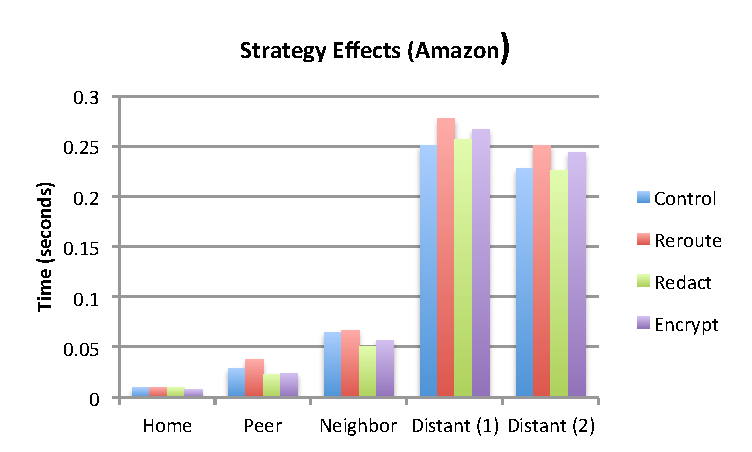
\includegraphics[width=6in]{strategy_effects_az}
%\caption{Hierarchical Results from Amazon}
%\label{fig:model:amazon-results}
%\end{figure}

\begin{figure}[htbp]
\begin{minipage}[b]{0.5\linewidth}
\centering
\subfigure[Mean Response Times]{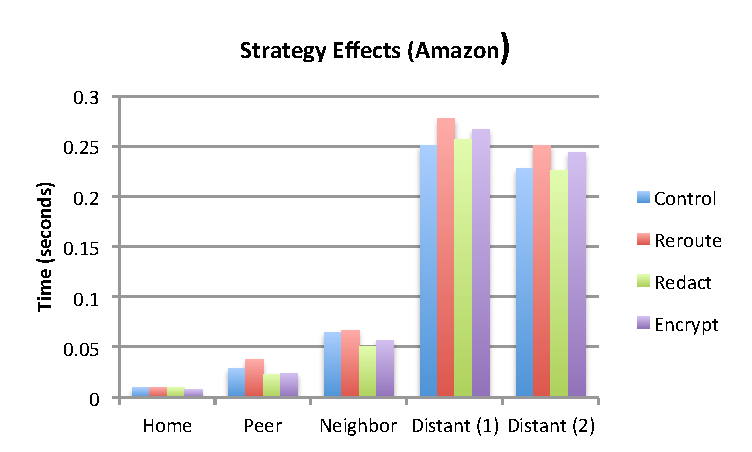
\includegraphics[width=\linewidth]{strategy_effects_az}}
\end{minipage}
\begin{minipage}[b]{0.5\linewidth}
\centering
\subfigure[Standard Deviation of Response Times]{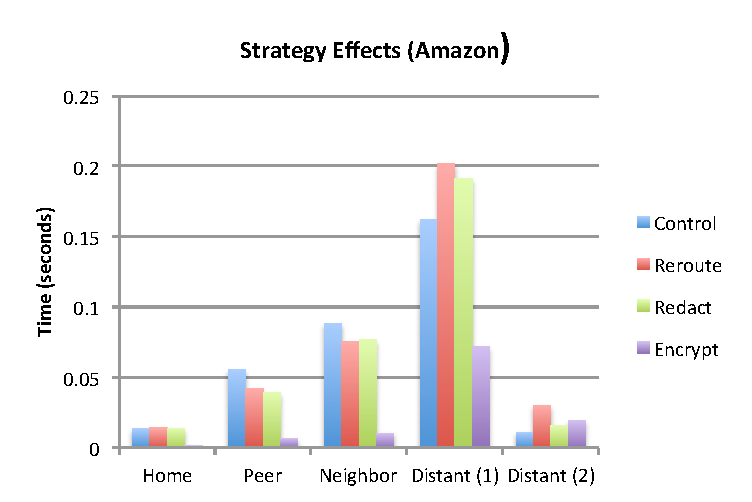
\includegraphics[width=\linewidth]{strategy_effects_stdev_az}}
\end{minipage}
\caption{Hierarchical Results from Amazon}
\label{fig:model:amazon-results}
\end{figure}

Figure ~\ref{fig:model:amazon-results} shows performance results from the Amazon testing node.  The access times for the content from the home, peer, and neighbor nodes were by far the smallest.  As the testing node was hosted in the same datacenter as these three nodes, that was to be expected.  The access times for both distant nodes was, however, surprisingly high.  With that in mind, the overall trend for response times is sensible however, with access time increasing as the requesting node is farther away from the content in the information network.  Queries from distant nodes need to traverse five information routers, while home, peer, and neighbor nodes only traverse one, two and three, respectively.  Also surprising was the finding that rerouting was generally more expensive from an availability perspective than encryption-based approaches.  This is likely attributable to the costs associated with attaching to the external SMTP server, hosted at Google, used as the out-of-band communications channel.  Also evident is remarkable performance variability.  Control data was collected at different times than experimental data, and infrastructural demands seem to have driven the control data availability to be less than that of other, managed approaches.  Overall, this evidence of variable performance due to external provider demands leads to the conclusion that overall, the availability costs of the various approaches are in fact negligible.

%\begin{figure}[!t]
%\centering
%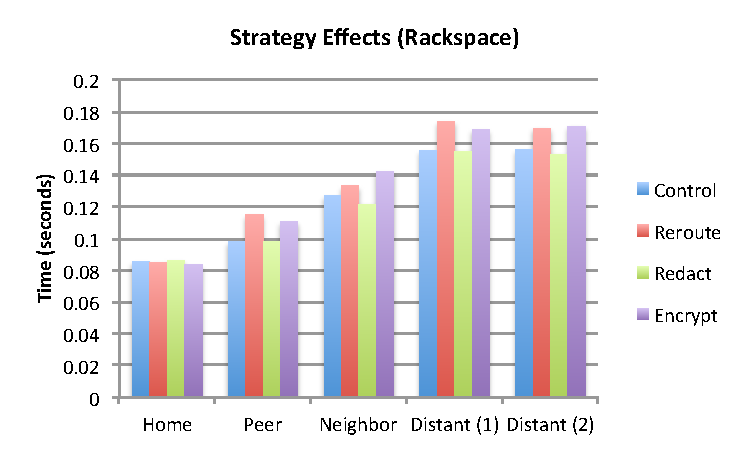
\includegraphics[width=6in]{strategy_effects_rs}
%\caption{Hierarchical Results from Rackspace}
%\label{fig:model:rackspace-results}
%\end{figure}

\begin{figure}[htbp]
\begin{minipage}[b]{0.5\linewidth}
\centering
\subfigure[Mean Response Times]{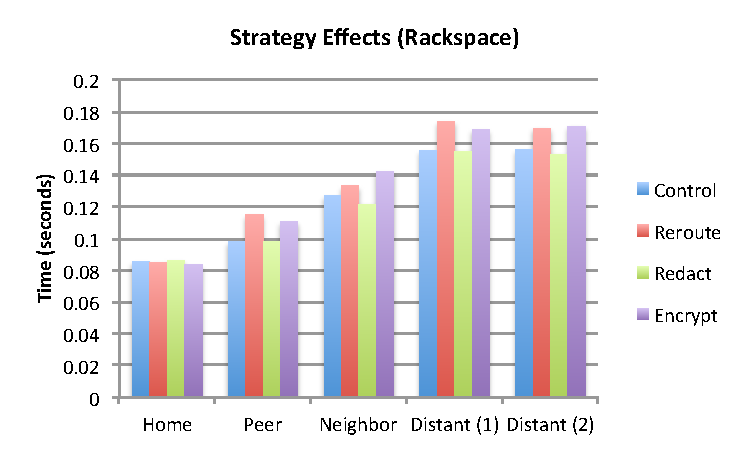
\includegraphics[width=\linewidth]{strategy_effects_rs}}
\end{minipage}
\begin{minipage}[b]{0.5\linewidth}
\centering
\subfigure[Standard Deviation of Response Times]{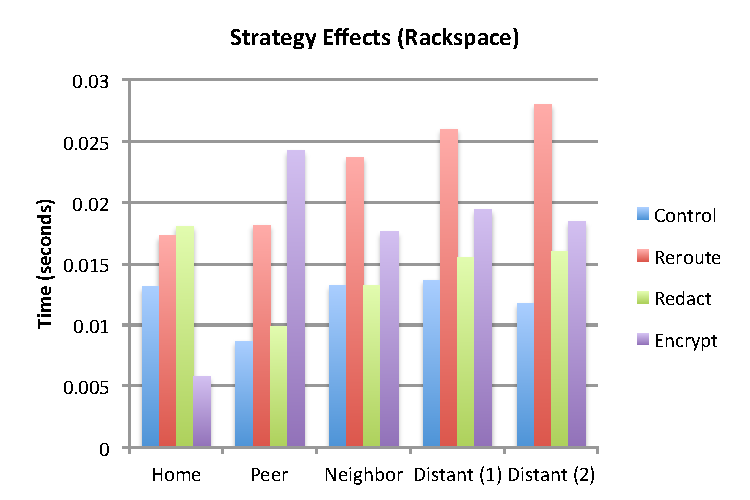
\includegraphics[width=\linewidth]{strategy_effects_stdev_rs}}
\end{minipage}
\caption{Hierarchical Results from Rackspace}
\label{fig:model:rackspace-results}
\end{figure}

Figure ~\ref{fig:model:rackspace-results} shows similar results to Figure ~\ref{fig:model:amazon-results}.  Here, the query times are much higher for the home and peer nodes, but actually lower for the distant nodes.  In this case, the content is still hosted in Amazon's infrastructure, but the testing node is at Rackspace.  As a result, the longer response time for content from the home node is to be expected.  Queries to distant nodes are actually shorter than the previous calls into distant nodes from Amazon.  This stems from the fact that the distant nodes are both hosted at Rackspace.  This locality shortens the round trip distance for a request.  Previously, from Amazon, a content request would need to travel from Amazon's east coast data centers to the Rackspace data center in Dallas, then back to the east coast for content, then back to Dallas, then back to the east coast.  In this test, the request only travels from Dallas to the east cost, and back.  Nevertheless, the overall performance profile is sensible, reflecting the expected shorter latency between home, peer, and neighbor nodes when compared to distant nodes.  Similar to amazon, cases when the control latency is higher than experimental latency emerge, indicating some amount of infrastructure performance variability.  In Figure ~\ref{fig:model:rackspace-results} however, it is evident that overall encryption and rerouting impact performance more than redacting, as would be expected.  Rerouting again has high overall impact, likely as a result of contacting Google's remote SMTP services.

Figure ~\ref{fig:model:comcast-results} Shows performance results measured from Comcast.  Interestingly, they show significant variability when accessing nodes hosted at Amazon, and more predictable performance when accessing nodes in Rackspace's infrastructure.  The overall variability does not follow the expected pattern of shorter response times when accessing content from nodes close to that content, except in a few cases.  This illustrates the kind of performance variability one can expect from an external service provider.

Integrity impacts are the result of approach rather than platform.  Redacting content destroys information integrity, as information is removed and not delivered to requesters.  Encryption maintains integrity the best of the three alternatives as information, even though encrypted, is still delivered, and delivered in the context of the query response at that.  Rerouting is better than redaction, in that sensitive information is still delivered, but worse than encryption, as it is not delivered within the response context and is sent out-of-band. Simulations removed sensitive information from the information network and dispatched it to a user's email address via SMTP over TLS when the selected strategy was rerouting.  This impacts information availability, as email delivery times can be highly variable.  In these experiments, delivery could take anything from a few seconds to a few minutes.

%\begin{figure}[!t]
%\centering
%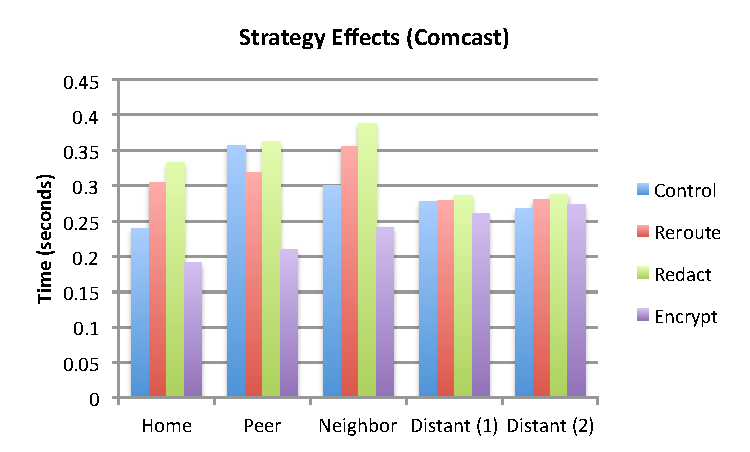
\includegraphics[width=6in]{strategy_effects_local}
%\caption{Hierarchical Results from Comcast}
%\label{fig:model:comcast-results}
%\end{figure}

\begin{figure}[htbp]
\begin{minipage}[b]{0.5\linewidth}
\centering
\subfigure[Mean Response Times]{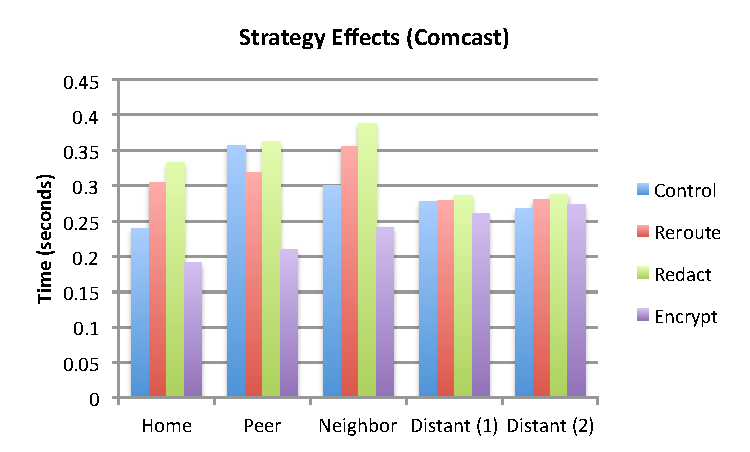
\includegraphics[width=\linewidth]{strategy_effects_local}}
\end{minipage}
\begin{minipage}[b]{0.5\linewidth}
\centering
\subfigure[Standard Deviation of Response Times]{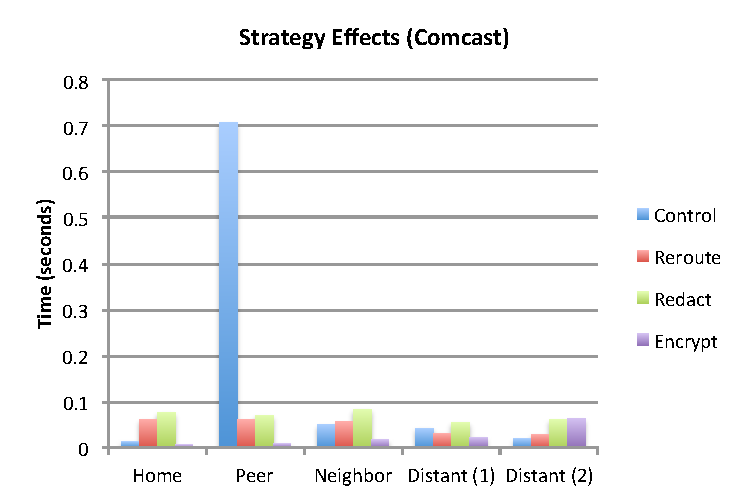
\includegraphics[width=\linewidth]{strategy_effects_stdev_local}}
\end{minipage}
\caption{Hierarchical Results from Comcast}
\label{fig:model:comcast-results}
\end{figure}

Confidentiality is likewise impacted primarily by approach and not by infrastructure.  Redacting sensitive content provides the best confidentiality protection, as sensitive content is simply not exposed.  Encryption is likely the worst solution from a confidentiality perspective as content encryption is a delaying tactic against a determined, well-resourced adversary.  Rerouting may be better or worse than encryption as an approach, depending on the confidentiality of the out-of-band channel.  If the security of that channel can be guaranteed, then it is likely a better approach.  If, on the other hand, the security of that channel is more variable or difficult to ascertain, encryption may be a more reliable approach.

Overall, results show that, from a performance perspective, the rerouting approach fares the worst, but only slightly, and certainly not in all cases.  Both results from Amazon and Rackspace, in Figures ~\ref{fig:model:amazon-results} and ~\ref{fig:model:rackspace-results}, show encryption as generally taking the second largest performance hit, just following rerouting.  Furthermore, network effects have a much larger impact on performance than information protection approaches.  The query to the home node is an excellent predictor of overall network stability, as content delivered directly from a home node is only subjected to the selected information protection strategy once.  Note that when queried from Amazon or Rackspace, the home node timing results are very close to uniform.  Queries from Comcast, however, are much more varied, indicating more highly variable quality of service within the Comcast network.  This is also supported by the gross distribution of response times.  Within both the Amazon and Rackspace networks, the farther a queried node is from the content requested, the worse the latency, as expected.  Comcast's network has a much more uniform information network response time overall as the processing time of the information network simulation is overshadowed by the highly varied performance of Comcast's physical network.  Availability is surprisingly uniform across all confidentiality strategies, showing little impact on end-to-end processing times.

\section{Non-Hierarchical Networks}
In order to test non-hierarchical networks, a simple branching network of participants was used, identical in form to the hierarchical network, though queries could be routed through the network from any point.  Queries could come into any node on the network, and would propagate through the network to the requested content, evaluating the returned content as it passes back through the network in response to the initial query.

In these experiments, the node that contains the content was queried, then the node immediately next to that content node, and so on, to a distance of five nodes.  The home node again contains content, and the additional nodes are marked by the distance in node count from the home node, starting with Neighbor (1), proceeding through Neighbor (5).  The non-hierarchical network was queried from Rackspace, Amazon, and Comcast, for a total of 250 queries per test, testing the system once per each confidentiality strategy.  Here, each figure is the result of 1500 individual sample measurements, again collected throughout the day and throughout the week.

%\begin{figure}[!t]
%\centering
%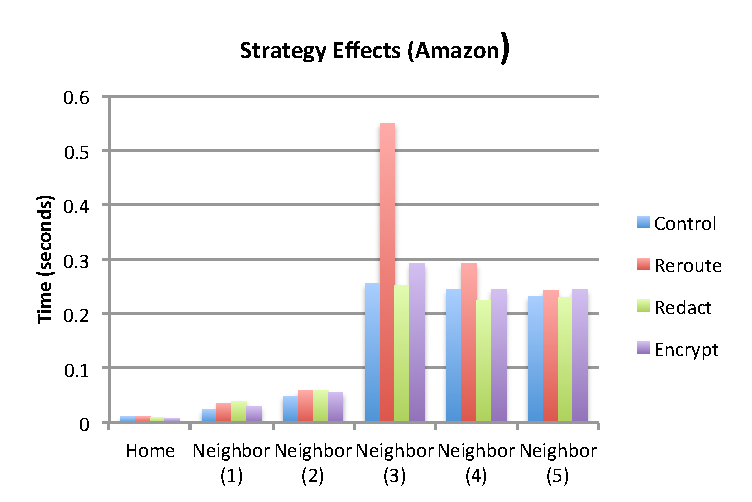
\includegraphics[width=6in]{nh_strategy_effects_az}
%\caption{Non-Hierarchical Results from Amazon}
%\label{fig:model:nh-amazon-results}
%\end{figure}

\begin{figure}[htbp]
\begin{minipage}[b]{0.5\linewidth}
\centering
\subfigure[Mean Response Times]{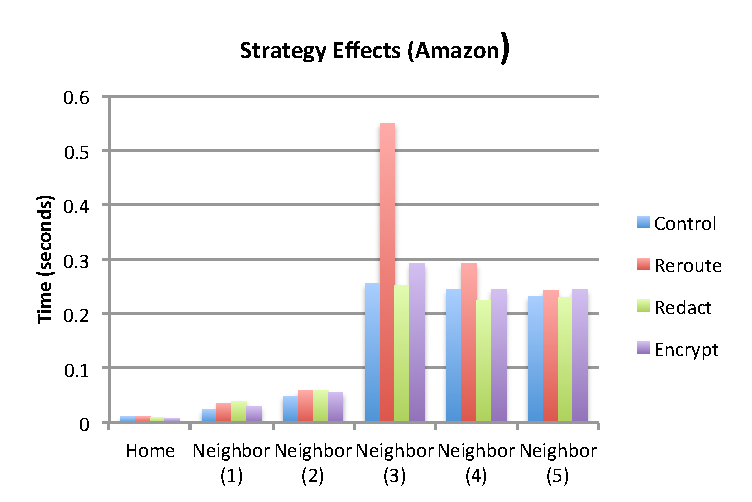
\includegraphics[width=\linewidth]{nh_strategy_effects_az}}
\end{minipage}
\begin{minipage}[b]{0.5\linewidth}
\centering
\subfigure[Standard Deviation of Response Times]{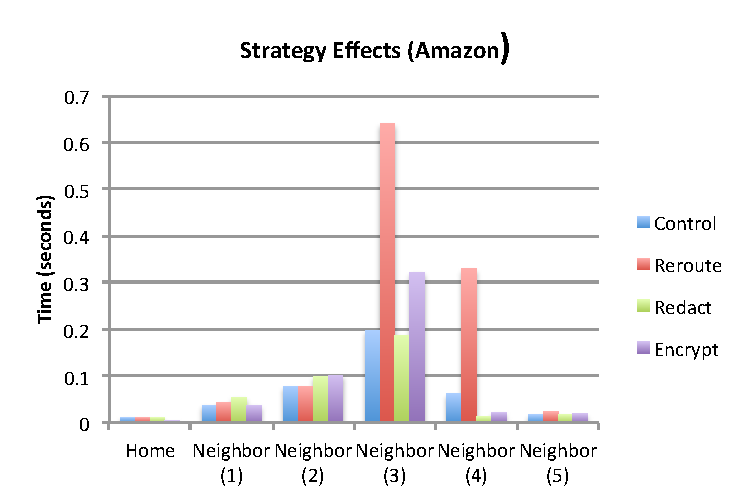
\includegraphics[width=\linewidth]{nh_strategy_effects_stdev_az}}
\end{minipage}
\caption{Non-Hierarchical Results from Amazon}
\label{fig:model:nh-amazon-results}
\end{figure}

Figure ~\ref{fig:model:nh-amazon-results} shows the performance of a non-hierarchical network as tested from the Amazon test node.  The content response latency is characteristic of moving farther from the source node through the network.  The request nodes switch from Amazon infrastructure to Rackspace infrastructure starting with Neighbor (3), and this is reflected in the sudden increase in latency.  As the tests originate from Amazon, at the Neighbor (3) node, a request and it's response must travel from Virginia to Texas, then back to Virginia, then back to Texas, then back to the original requester in Virginia.  The spike in latency at Neighbor (3) when re-routing traffic is caused by SMTP delays with systems hosted at Google.  Overall, the distribution is very similar to the hierarchical case.  Also evident is a continuation of the previous pattern in which re-routing is the least efficient strategy, followed by encryption, then redaction.

%\begin{figure}[!t]
%\centering
%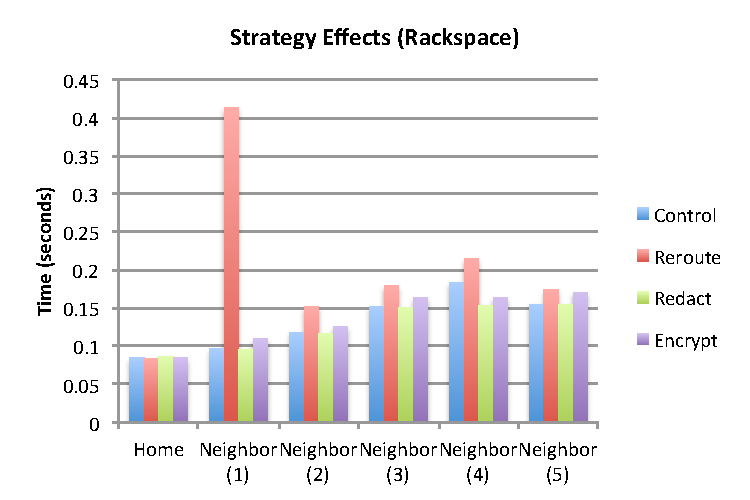
\includegraphics[width=6in]{nh_strategy_effects_rs}
%\caption{Non-Hierarchical  Results from Rackspace}
%\label{fig:model:nh-rackspace-results}
%\end{figure}

\begin{figure}[htbp]
\begin{minipage}[b]{0.5\linewidth}
\centering
\subfigure[Mean Response Times]{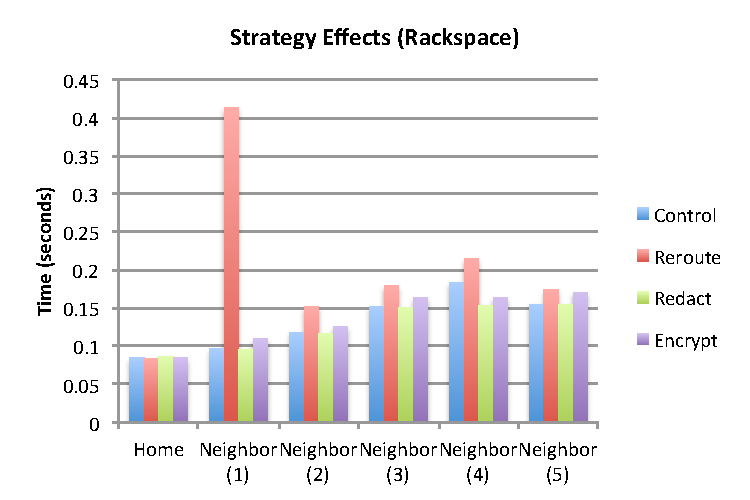
\includegraphics[width=\linewidth]{nh_strategy_effects_rs}}
\end{minipage}
\begin{minipage}[b]{0.5\linewidth}
\centering
\subfigure[Standard Deviation of Response Times]{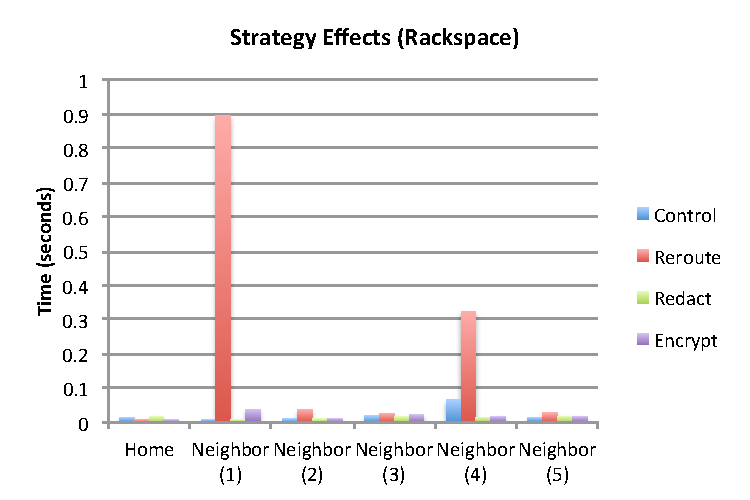
\includegraphics[width=\linewidth]{nh_strategy_effects_stdev_rs}}
\end{minipage}
\caption{Non-Hierarchical Results from Rackspace}
\label{fig:model:nh-rackspace-results}
\end{figure}

Unlike the previous Amazon-based tests, the Rackspace tests shown in Figure ~\ref{fig:model:nh-rackspace-results} latencies seem much more uniform.  This again stems from the fact that each content query will always traverse the distance between Amazon and Rackspace data centers at least once.  Other than that, the distribution again shows an increase in measured latency as the queried node moves farther and farther away from the home node.  Once again, a dramatic spike in latency emerges based on SMTP delays when re-routing information.  The pattern of re-routing having the highest latency continues here as well.

%\begin{figure}[!t]
%\centering
%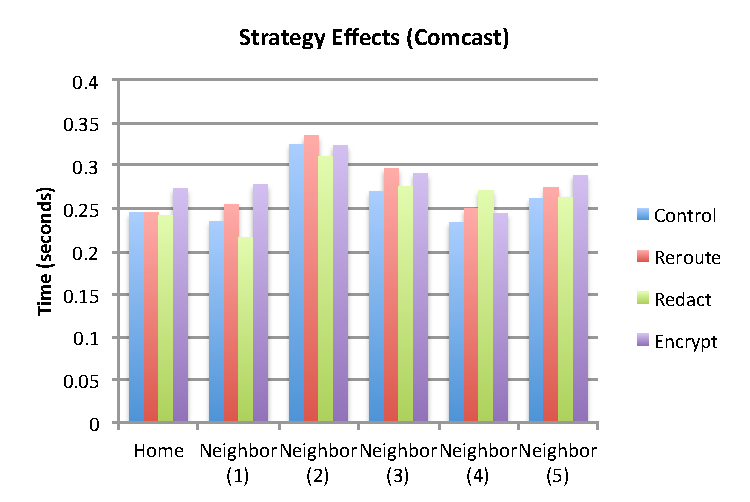
\includegraphics[width=6in]{nh_strategy_effects_local}
%\caption{Non-Hierarchical Results from Comcast}
%\label{fig:model:nh-comcast-results}
%\end{figure}

\begin{figure}[htbp]
\begin{minipage}[b]{0.5\linewidth}
\centering
\subfigure[Mean Response Times]{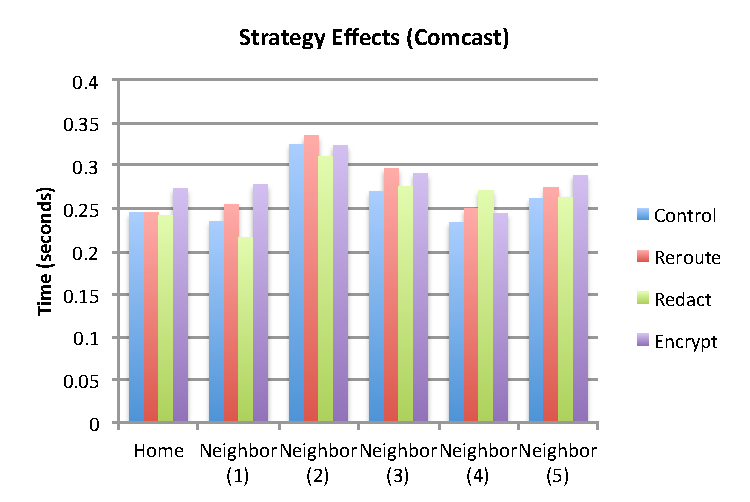
\includegraphics[width=\linewidth]{nh_strategy_effects_local}}
\end{minipage}
\begin{minipage}[b]{0.5\linewidth}
\centering
\subfigure[Standard Deviation of Response Times]{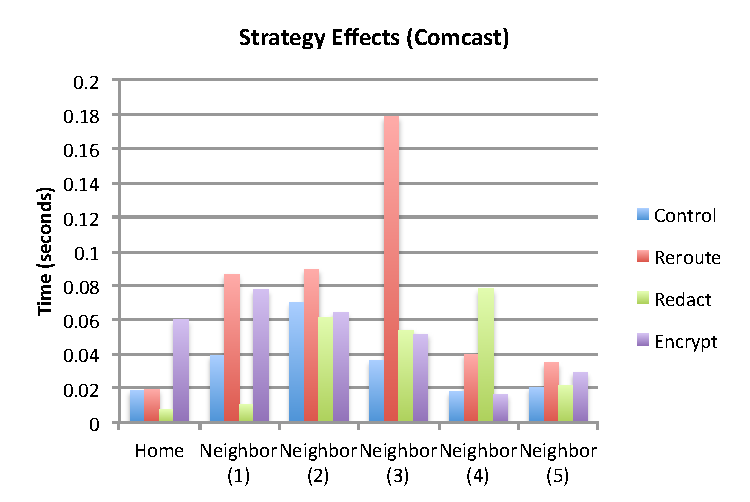
\includegraphics[width=\linewidth]{nh_strategy_effects_stdev_local}}
\end{minipage}
\caption{Non-Hierarchical Results from Comcast}
\label{fig:model:nh-comcast-results}
\end{figure}

Results from Comcast, included in Figure ~\ref{fig:model:nh-comcast-results}, shows a fairly regular distribution of response latencies overall.  In this case, the test node is ensconced within Comcast's network infrastructure.  Generally, re-routing is the least efficient approach, but not uniformly.  In this case, network effects created by the physical location of the testing node dominate these results.

Non-hierarchical networks behave very similarly to hierarchical networks.  This is not surprising --- although the nodes are more functionally complex, performing routing and repository functions, once the content is found and delivered the roles the nodes fall into mirror those in a hierarchical network.  For example, in a typical query, a node will receive a request, check the repository for the requested content, and if the content does not exist, pass the request onto the next known nodes.  This does differ slightly from the hierarchical case in that the nodes check for content at each routing step, though this is a very fast and simple test.  Once content is found, the response is routed back the the requester without any repository checks, just as it would be in a hierarchical system.

\section{Removing Network Effects}
Having established the parameters under which confidentiality strategies may be chosen, the next immediate area of concern involves the number of filtering events that can occur prior to a given information network suffering from degraded performance.  Previous results demonstrated that some kind of degradation of performance in the selected network based on distance from content does exist, but that can also be attributed to the distributed nature of the network itself.  Processing performance of a given node must be evaluated free of network effects in order to more clearly understand the availability implications of content filtering itself.

A single node, configured on one of the test nodes in either infrastructure, would yield the type of network effect free performance limits needed.  A node in Amazon's environments was configured such that requests were made of the home node itself, under each of the three confidentiality strategies.  Requests were also directed to the home node without any usage management systems engaged in order to collect control data.  After that initial request, the node was configured with various usage management strategies in order to measure their availability impact.

%\begin{figure}[!t]
%\centering
%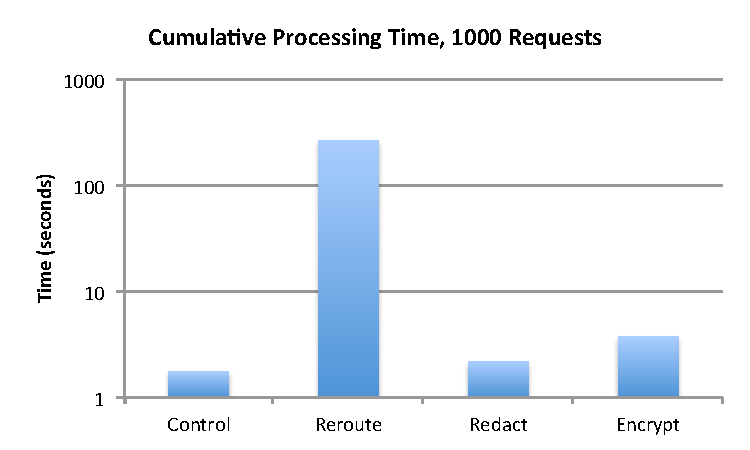
\includegraphics[width=6in]{single-node-results}
%\caption{Results from Requests to a Singe Node}
%\label{fig:model:single-node-results}
%\end{figure}

\begin{figure}[htbp]
\begin{minipage}[b]{0.5\linewidth}
\centering
\subfigure[Mean Response Times]{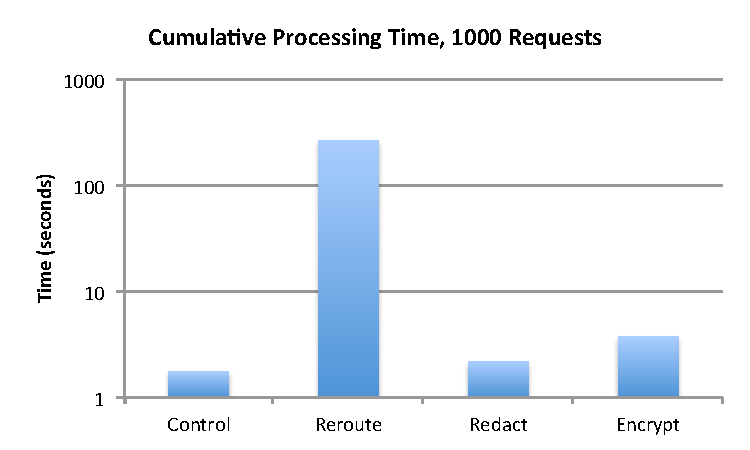
\includegraphics[width=\linewidth]{single-node-results}}
\end{minipage}
\begin{minipage}[b]{0.5\linewidth}
\centering
\subfigure[Assorted Other Statistics]{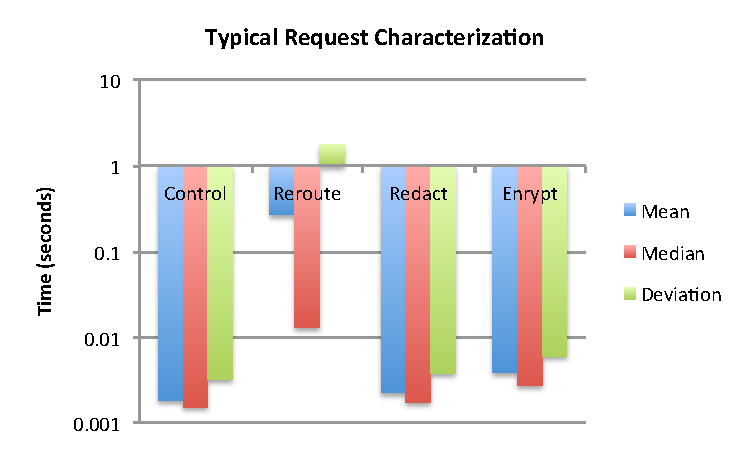
\includegraphics[width=\linewidth]{single-node-results-stats}}
\end{minipage}
\caption{Non-Hierarchical Results from Rackspace}
\label{fig:model:single-node-results}
\end{figure}

As shown in Figure ~\ref{fig:model:single-node-results}, with information network effects removed, redaction and encryption have very similar performance overall.  Redaction, as a strategy, is very simple programmatically, and as symmetric encryption is used for information protection, ciphering and deciphering operations are very fast.  Rerouting, in this case, is clearly the worst strategy.  This is a result of the dependency of this strategy on external systems and system configuration times.  Specifically, configuring and using SMTP for each rerouting operation is prohibitively expensive.